% Kapitel 3

\chapter{Data Efficiency in Neural Network-Based Image Segmentation}
\label{chap:data-efficiency}

Above all, the accuracy of neural networks is governed by three factors: problem complexity, number of network parameters, and size of the dataset. All of these factors contribute to accuracy in different ways and there is a complex interplay between them. To understand data efficiency, it is key to clearly understand these concepts. We will begin this chapter by exploring neural networks as function approximators. We still start with a simple example of a neural network and build an understanding of the four factors in general terms. After that, we will expand our example to include image segmentation.

Let us consider a statistical learning problem of estimating the 10-year risk of heart disease given age. In this case, there exists some unknown underlying dependency between age and risk of heart disease. However, there is no way to know what this function is. All we can do is collect a set of data points and try to approximate a function that explains those data points. In other words, we want to find a curve that tries to minimize some criterion that takes into account the distance between the curve and the collected data points.

There are an infinite number of functions that can minimize this criterion. Therefore, we have to choose a class of functions to evaluate. One of the simplest classes of functions we could use are lines --- leading to a simple linear regression. A line is defined by two parameters, its slope $\theta_1$ and intersect $\theta_0$:

\begin{equation}
	f(x) = \theta_1 x + \theta_0
\end{equation}

Here, $f(x)$ is our regression model. Our goal is to find the optimal values of $\alpha$ and $\beta$ that best explain the collected data samples in the form of $(x_i, y_i)$. We can do so by minimizing the mean squared distance between the line and each data point:

\begin{equation}
	\min_{\theta_1, \theta_0} \sum_{i=1}^N (y_i - f(x_i))
\end{equation}

Given a set data points, we will use the above equations to fit a line between them. In \figref{fig:slr-points} we show this line for a different number of datapoints. As can be seen, the number of samples impacts the results drastically. As is intuitive, more samples gives us a line that better matches the real data distribution.

\begin{figure}[h!]
 \hfill
 \subfloat{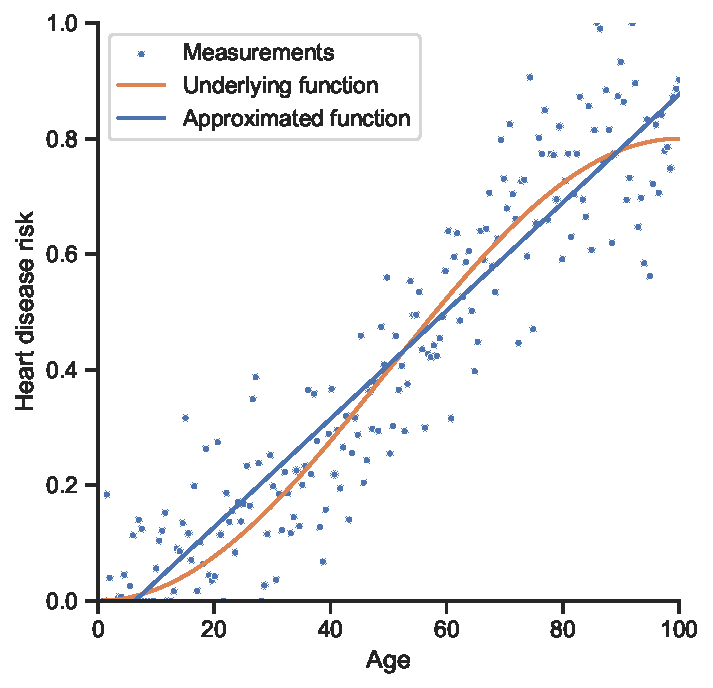
\includegraphics[width=0.5\linewidth]{images/3/heart_disease_risk}}
 \hfill
 \subfloat{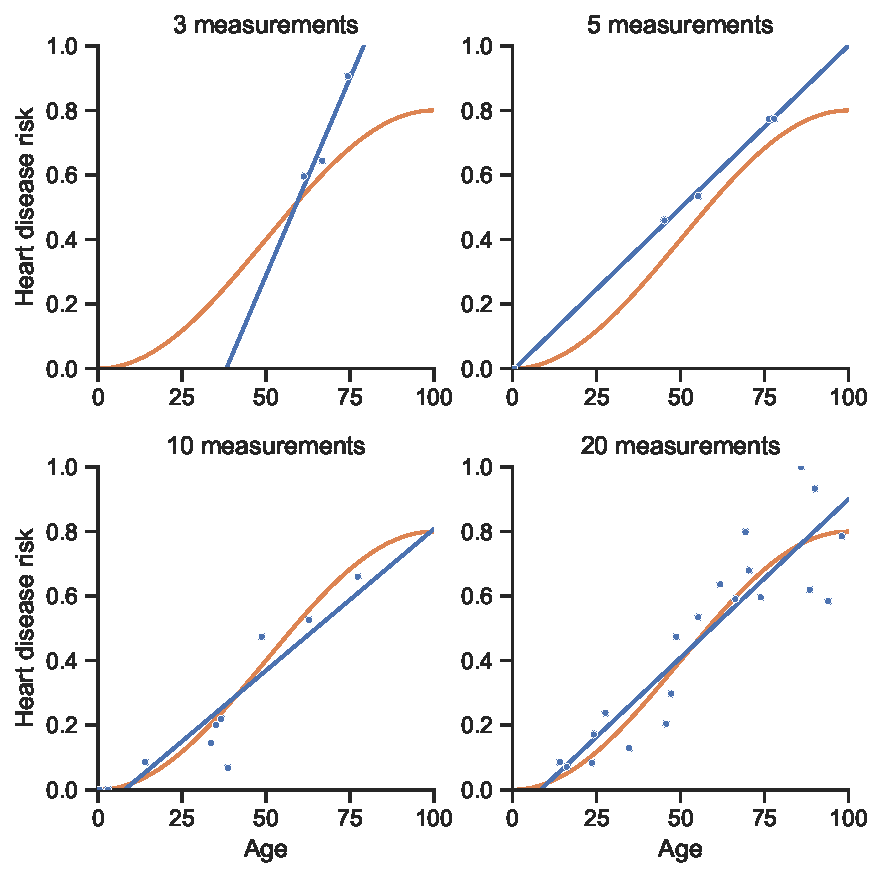
\includegraphics[width=0.5\linewidth]{images/3/heart_disease_risk_samples}}
 \hfill
 \label{fig:t1-t2-example}
 \caption{A simulated example of heart disease risk prediction using simple linear regression. The plots on the right show how the approximated function depends on the sample size.}
\end{figure}

Clearly, having only three points results in an approximated function that does not match the underlying one. As we increase the sample size, the approximated function becomes much closer to the underlying one. However, note that even for 20 measurements, the linear function differs from the underlying one. The underlying function is a non-linear cosine function. Even with infinitely many data points, our function will never approximate the underlying function perfectly with just two parameters.

To overcome this, we need a more complex model. We can think of our regression so far as fitting a polynomial function to our dataset. For the initial example, we have used polynomials with a degree of 1 --- lines. We can generalize our function to an $n$-degree polynomial as:

\begin{equation}
	f(x) = \theta_n x^n + \theta_{n-1}x^{n-1} + \cdots + \theta_1 x + \theta_0
\end{equation}

To model heart disease risk, we will choose a polynomial degree $n$ and minimize the mean squared distance to obtain $\theta_n$ through $\theta_0$. By increasing the degree increasing the complexity of the model, i.e. the model will be able to represent more complex curves than simple lines. We can observe what happens when we choose degrees 2, 3, or 5 in \figref{fig:reg-deg-2}.

\begin{figure}[h!]
 \centering
 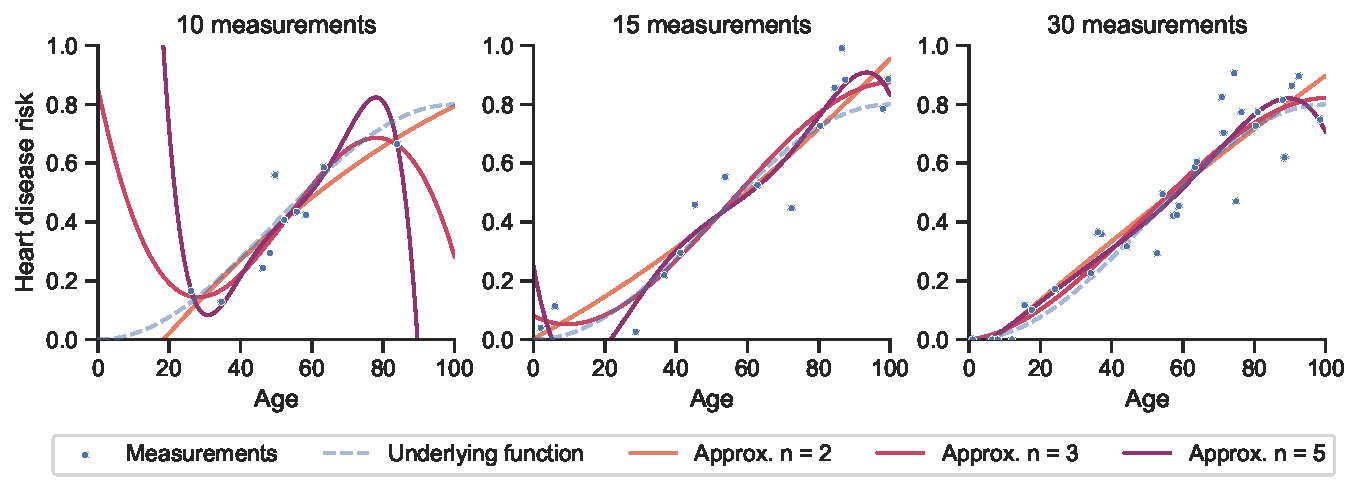
\includegraphics[width=\linewidth]{images/3/heart_disease_risk_samples_degrees}
 \caption{Fitting a polygonal function of various degrees on three different sample sizes.}
 \label{fig:reg-deg-2}
\end{figure}

When looking at the example with 10 measurements, we can see that for $n = 2$ the approximated polynomial follows the underlying function somewhat well. However, as we increase the degree the function quickly deteriorates. This is called \textbf{overfitting} --- the model has fit a particular sampling of the data but does not generalize to unseen examples. In other words, the model is impacted by the noise present in the training set. This is contrasted by \textbf{underfitting}, where the model does not have enough parameters to fit a complex function, as exemplified by our linear model in Figure \ref{fig:t1-t2-example}.

This fundamental problem is called the bias--complexity tradeoff (or sometimes the bias--variance tradeoff). Formally, as shown in \todo{cite ML book}, we can decompose the error of a deep learning model into two components. Let there be a function $L(f)$ that measures the error of some model $f$ compared to the true function we are approximating. Assume that our trained model $f_\theta$ with parameters $\theta$ comes from a class of functions $F$. The error of such a model can be expressed as:

\begin{equation}
	L(f_\theta) = \epsilon_{app} + \epsilon_{est}
	\text{ where:\;}  \epsilon_{app} = \min_{f \in F}L(f),\;
	\epsilon_{est} = L(f_\theta) - \epsilon_{app},
\end{equation}

where $\epsilon_{app}$ is the \textbf{approximation error} and $\epsilon_{est}$ is the \textbf{estimation error}. The approximation error represents the error we are left with when we use the best possible estimator within our class of functions $F$. In the earlier example of function approximation, when use used a 1st degree polynomial, even given infinite data we would always have some error compared to the underlying function. The approximation error depends entirely on the class of functions we use, and can only be changed by using a different class of functions, such as higher-degree polynomials.

The remainder of the error depends on the quality of our parameters $\theta$. It is possible to choose a class of functions that can perfectly approximate the underlying function and still not correctly approximate it due to a difference in the underlying and trained parameters. As we saw in earlier examples, this error depends heavily on the data sample we have. A small or unrepresentative sample is bound to give a poor estimate of optimal parameters.

We can investigate the bounds of the estimation error so see what it depends on. We can do so by using the concept of \textbf{sample complexity}. In this context, sample complexity $n(\epsilon, \delta)$ for chosen $\epsilon, \delta \in (0, 1)$ measures how many samples we need in order for some function $f$ chosen from a finite class of functions $F$ to be correct within $\epsilon$ with a probability of $1 - \delta$, or in other words:

\begin{equation}
	L(f) \leq \epsilon.
	\label{eq:erm-hyp}
\end{equation}

Assuming there exists some unknown $f' \in F$ for which $L(f') = 0$, it can be shown \todo{cite ml book page 41} that (\ref{eq:erm-hyp}) holds if:

\begin{equation}
	n(\epsilon, \delta) \geq \frac{\log(\lvert F \rvert \delta)}{\epsilon}.
\end{equation}

In other words, as we increase the size of the function class $|F|$ (in other words, make our model more complex), we need a larger sample size $n$ to approximate the underlying function. Going back to our error decomposition from earlier, we see that if we restrict the model complexity too much, we will suffer from a high approximation error or underfitting. On the other hand, as we increase the model's complexity, we have a higher requirement for data and a greater chance of overfitting. 

A third component is the complexity of the underlying function. If the underlying truly resembles a line, then it can be successfully approximated using a few parameters. However, most problems in medical image segmentation involve very complex high-dimensional functions and thus require very complex models to usefully approximate the functions. 

Thus, in medical image segmentation we have an unfortunate stalemate between three interdependent conditions. Medical image segmentation is complex and requires a large number of parameters. Having a large number of parameters requires sufficient data samples for the model to be probably approximately correct. However, we usually do not have a sufficient amount of samples. Therefore, we need methods to reduce the estimation and approximation errors other than adding more data samples for the problem at hand.

Approximation error can be decreased by using a less restrictive class of functions. However, when dealing with neural networks and small datasets, approximation error is typically small since neural networks naturally have access to a very large class of complex functions. Instead, the focus should be on reducing estimation error. The easiest way to do so would be to increase the sample size. However, we have already mentioned that this is infeasible in medical image segmentation. Therefore, we need to leverage other methods of reducing the estimation error.

The we way can achieve a lower estimation error is by reducing the class of functions the final model needs to optimize over. We can do so in two directions. One, we can reduce the parameters of the model itself. The class of functions is then smaller and the model can more easily find the optimal function. This usually requires transforming the data such that it can be easily segmented with a less complex function. Two, we can initialize the model with near-optimal parameters. The model is then already in the neighborhood of the optimal function, and only needs to search a local space near the given parameters. This latter method usually requires optimizing a model on similar data using a task that requires learning features relevant for segmentation. We then take the pre-optimized parameters and optimize them further for the segmentation task at hand.

The first method -- transforming the data -- leverages domain knowledge to guide transformations of the image beneficial to segmentation. However, these transformations are deterministic and therefore have a limited understanding of the contents of the image. It is hard to adapt them to each subject and different locations of the target tissue to be segmented. The second method can better handle these dynamic image features, but still requires a sufficient amount of data that is similar enough to the downstream segmentation task. In the following sections, we will cover these methods in detail with examples of how they are used in neural network-based medical image segmentation.

\section{Transfer Learning}

Transfer learning is the process of initializing the parameters of one neural network with those of another. For instance, we might be dealing with the problem of segmenting liver tumors on CT scans. We have a limited number of labeled liver tumor regions but a larger number of labeled liver regions. Therefore, we first train a neural network for liver segmentation. We assume that the majority of the parameters learned by the network are close to the ones needed for liver tumor segmentation. Therefore, when we are developing the liver tumor segmentation network, we copy the valus of the parameters learned in the liver segmentation network. We then say that the network was \textbf{pre-trained} or \textbf{initialized} on a liver segmentation dataset and \textbf{fine-tuned} on the liver tumor segmentation dataset.

This example, where we use transfer learning from one related segmentation task to another is usually referred to as just transfer learning. However, transfer learning can also be achieved using much more complex methods of pre-training. Therefore, in this thesis, we use the term simple transfer learning to referer to this basic method. Other methods include semi-supervised learning as well as domain adaption, which will be described later in this section.

	\subsection{Simple Transfer Learning}
	
Simple transfer learning is used extensively in medical image segmentation. Segmentation neural networks are commonly initialized using weights trained on the ImageNet dataset \todo{cite}. ImageNet is a dataset of natural images and its distribution is drastically different from medical images. Therefore, this initialization does not typically lead to increases in accuracy, but can make the network converge faster as it ``skips'' having to learn to detect base-level image features common to all images.

\todo{diagram here}

However, there are more recent datasets \cite{wasserthalTotalSegmentatorRobustSegmentation2023} that include >1000 subjects and are commonly used for transfer learning, improving the accuracy of downstream tasks \cite{monaiconsortiumMONAIMedicalOpen2023, myronenkoAutomated3DSegmentation2023}. While these approaches can result in impressive performance improvements, their use is limited to areas where a sufficient amount of similar data is available. For more niche modalities or segmentation problems, the knowledge learned during pre-training can be insufficient to improve the accuracy of the task at hand. One way to alleviate this issue is to somehow adapt the pre-trained model to the target domain. We will discuss this next.

	\subsection{Domain Adaptation}
	
Neural networks trained on one dataset often fail to generalise to other datasets, even within similar domains \cite{torralbaUnbiasedLookDataset2011}. This is referred to as the ``domain shift'' problem. Overcoming this problem could lead to an increase in data efficiency, since a model trained on some similar large dataset can perform well on a smaller target dataset. There are various domain adaptation methods that aim to overcome the domain shift problem.

There are several ways to achieve domain adaptation. One class of methods aims to explicitly penalize domain shift by including an estimate of domain shift in the loss function during training. For instance, \citet{liuUnsupervisedDeepDomain2018} use an approach where they first train a network on a source domain where there is a large amount of data available. This network is then used to perform segmentation on a target domain with a low amount of data. During the adaptation phase, the loss function includes a maximum mean discrepancy term between the encoded feature vectors of the source and target domains. By minizing maximum mean discrepancy, the encoder is forced to keep producing feature representations from a constant distribution, instead of shifting the distribution.

Another class of methods focuses on minimizing a network's ability to differentiate between the source and target domains. For instance, \citet{ganinDA2015} add a parallel classification head to the network that aims to detect the domain of the input. Normally, during each iteration the network adjusts its parameters in such a way to reduce the loss. However, in \cite{ganinDA2015} the gradients of the domain classifier are inverted, and so the network updates its parameters to make it harder to differentiate between the two datasets. This approach can be seen in \figref{fig:unsup-dom-adpt}.

\begin{figure}[h!]
 \centering
 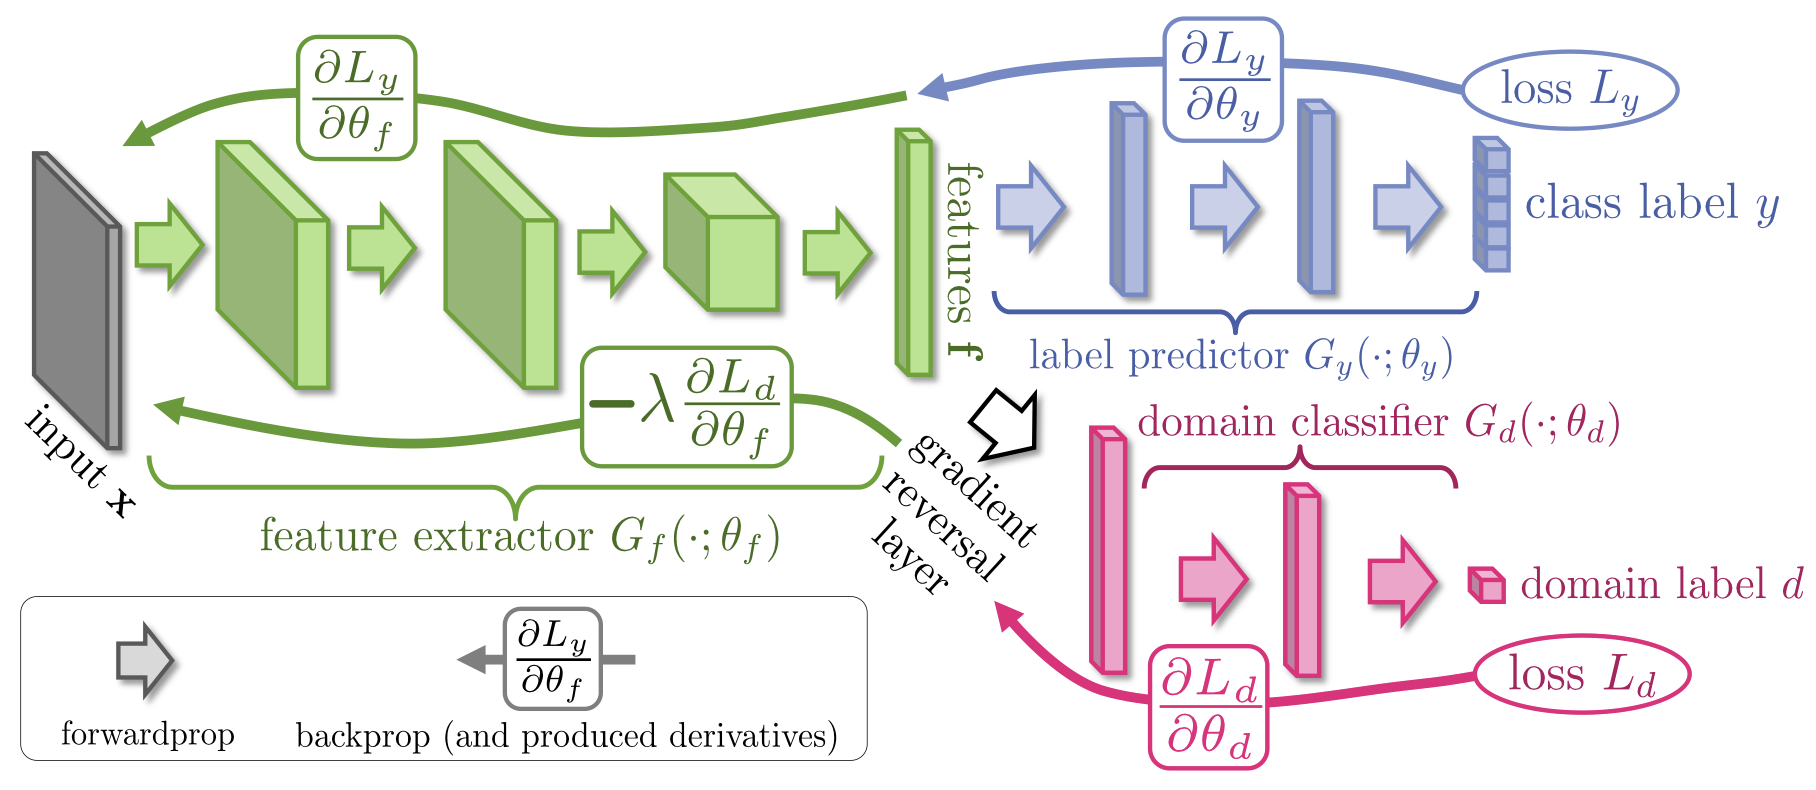
\includegraphics[width=0.7\linewidth]{images/3/unsup-dom-adpt}
 \caption{A diagram of the domain adaptation approach in \citet{ganinDA2015}. The gradients of the domain classification head which are applied to the encoder are reversed during backpropagation.}
 \label{fig:unsup-dom-adpt}
\end{figure}
	
Both approaches have been applied to medical image segmentation, such as in \citet{bermudez-chaconDomainadaptiveTwostreamUNet2018} where U-Net like architecture is used with two encoder branches. Each branch receives images of one image domain, and a shared decoder. The loss function includes a maximum mean discrepancy term between the decoder's final feature maps of inputs from the two domains. They apply their method to segmenting mitochondria and synapses in microscopic images. 

While allowing improvements in transfer learning performance, domain adaptation methods require labeled data for the source domain. Approaches which could leverage unlabelled data can learn to recognize features on images from the same domain as the segmentation task. We will discuss such approaches next.

	\subsection{Semi-Supervised and Self-Supervised Learning}
	
Semi-supervised learning involves the combination of labeled and unlabeled data to train a neural network. The network can use the unlabeled data to learn to extract general image features that are useful for the downstream segmentation task. This feature extractor is then employed to train the final network on the labeled target dataset. This makes the network more label-efficient, as it can effectively learn without having to label a large amount of data.

The goal of this approach is to train a feature extractor that has a general ability to extract salient features from the image. Even though the exact segmentation task is not known, one can construct synthetic tasks without requiring labels that would force the network to extract features.

One such approach is \textbf{self-supervised learning}, where a feature extractor can be trained in a completely unsupervised manner using a large number of images. Then, that feature extractor can used and fine-tuned in a downstream segmentation model to segment images similar to the ones the extractor was trained on.

SSL is a method of unsupervised neural network training where the
goal is to train an encoder that will understand useful features for a downstream
task such as object detection, classification, or similar. SSL has
been shown to improve data efficiency
\cite{chenSimpleFrameworkContrastive2020} as well as robustness to dataset imbalance
\cite{liuSelfsupervisedLearningMore2021}.

There are several approaches to training the encoder such that it learns useful features.
One approach is to use a constructed \textbf{pretext task} for which one
can automatically obtain the correct solution from unlabeled data so that the correct solution can be used
for supervised training. An example of this approach is presented by 
\citet{norooziUnsupervisedLearningVisual2016} where the neural network is trained to 
solve a jigsaw constructed from an unlabeled dataset. An image is cut into $3 \times 3$ tiles that are randomly shuffled to construct an input image. The task of the network is to reorder the tiles (i.e. solve the jigsaw puzzle) to reconstruct the original image. By solving this task, the network is forced to learn features of the image.

\todo{contrastive learning diagram maybe?}

Recently, a more common approach to SSL is \textbf{contrastive learning}.
In contrastive learning, the encoder is trained to minimize the distance between feature
vectors of positive examples and maximize the distance between negative examples. The
positive examples are constructed in an unsupervised manner by e.g. randomly augmenting
an image twice, thus producing two examples for which the feature vectors should be
similar. Among others, notable examples of such approaches are SimCLR 
\cite{chenSimpleFrameworkContrastive2020} and MoCo \cite{he2019moco}.

\section{Synthetic Data}

So far, the data efficiency methods discussed have been focused on pre-training the networks on unlabelled or similar data. However, an alternative approach would be to synthetically generate data from the target distribution. This can be achieved using techniques or varying complexity and generation quality. One of the simplest and most well-known ways of synthetically increasing the size of a dataset is \textbf{data augmentation}. 

\textbf{Data augmentation} involves applying randomized transformations to the input images to artificially increase their diversity. These transformations range from simple ones like changing brightness or contrast, horizontally mirroring the image all the way to more complex random deformations of the image. Data augmentation is commonplace in segmentation models and is usually in conjunction with other methods for data efficiency. However, it is usually implemented using simple deformation or transformation procedures and thus has limited ability to generate truly diverse samples.

Recently, the field of deep learning-based image generation, especially generative adversarial networks and diffusion models, have sparked a large interest in generating synthetic medical images. \todo{cite} 
% That paper with vessel segmentation with fractal generation

\section{Regularization}

As mentioned earlier, aside from getting new data, the easiest way to reduce the estimation error is by limiting the size of the function class our model optimizes. In a traditional machine learning approach, this would be done by hand-selecting a class of functions with a lower number of parameters and then training the model. In deep learning, however, this approach is usually replaced with regularization, where the parameters themselves are manipulated to simplify the model.\footnote{Often, any method of reducing the estimation error of a model is broadly termed as regularization.} Instead of selecting the number of parameters, we can penalize the network for the complexity and size of parameters. \todo{cite Deep learning book 7.1.1 https://www.deeplearningbook.org/contents/regularization.html} In other words, the loss function used during training has the form:

\begin{equation}
	L(\theta; I, y) = L_{seg}(\theta; I, y) + \alpha\Omega(\theta)
\end{equation}

where $L_{seg}$ is the segmentation loss function while $\Omega(\theta)$ is a parameter norm penalty, i.e. a measure of the complexity of the model. As we increase $\alpha$, the strength of the regularization increases and the loss is more impacted by the complexity of the model. As the network is being trained, it will seek to both reduce $\Omega(\theta)$ as well as $L_{seg}$, leading to a more constrained model.

A commonly used parameter norm penalty is the $L^2$ regularization, also known as \textbf{weight decay} in deep learning contexts. Assuming $\theta$ consists of a set of weights $w, |w| = n$ and biases $b$, the $L^2$ norm is defined as $\Omega(w) = \frac{1}{2}\sqrt{(w_1^2 + w_2^2 + \cdots + w_n^2)}$. In other words, the network is exponentially penalized for moving weights away from zero. This regularisation, in effect, forces the network to use as few parameters as possible to achieve its task.

\subsection{Conclusion}

As we have seen, there are a number of approaches to increasing the data efficiency of neural network-based segmentation of medical images. This thesis focuses on using regularisation by transforming the input data in such a way as to allow the network to use fewer parameters to achieve its segmentation task. We do so by combining predictions of neural networks with more traditional approaches from image processing and data augmentation. In the next chapter, we will introduce this idea and some specific applications.

%	\subsection{Leveraging Inductive Bias}
%	
%The core of achieving data and label efficiency is in manipulating the \textbf{inductive bias} of a model. If we are trying to approximate functions, we quickly run into a problem --- for any given set of finite points, we can find an infinite set of functions that can correctly approximate those points. Thus, we need to constrain the space of possible functions in some way. In the previous section, we assumed our functions were polynomial with a fixed number of degrees. That is an inductive bias --- we have biased our model to only consider polynomial relationships between the inputs and the labels.
%
%We can use inductive bias to our advantage. With a more constrained function space, the model can more easily converge to an optimal set of parameters. We have observed this effect in Figure \figref{fig:reg-deg-2}, where the 1 and 2-degree polynomials are able to closely fit the underlying function even with a few datapoints.
%
%We can also extend this to CNN architectures. Simply by using convolutions are their fundamental operation, a CNN has beneficial inductive biases for processing images. \todo{todo}
%	
%	\subsection{Transforming the Data}
	
%\section{Model-guided Transformations}

% todo in the book he mentions different feature representation
% 25.2 Feature Manipulation and Normalization

%When segmenting liver tumors in CT image, an expert, given a voxel location and image, can map each location to a probability of encountering a liver tumor on that image. They do so based on experience, intuition, and complex models of the real world including anatomy, pathology, biological processes of cancerous cell multiplication, understanding of how different vascular systems propagate contrast to cancerous and normal cells, etc. It is computationally infeasible to model these processes directly, so instead we opt for sampling a set of CT images and approximating the underlying processes as a continuous function.
%
%The sampled points are in the form of $(I(A), M(A))$ i.e. an image and segmentation map pair, as labeled by an expert. If we consider the image and segmentation map to be high-dimensional vectors, we can think of both as existing in a high-dimensional space.


%At their core, neural networks are function approximators. Every voxel in a CT scan contains either normal tissue or a liver tumor. Cancerous cells multiply and grow according to biological processes and are thus localized in specific areas. Because the cancerous cells are supplied with blood by the hepatic artery, an injected contrast reaches them sooner than normal cells, causing them to appear brighter in the image. These are just a few of infinitely many processes that govern the true probability of a voxel containing cancerous tissue. All of these processes together form an exceedingly complex function that maps a voxel its true probability of containing cancerous tissue. The goal of a segmentation network is to approximate this natural function using a statistical model. 
%
%We may imagine a CT scan as a point that lies in a high-dimensional space, where each voxel value is one dimension of the point.
%
%
%In image segmentation, this 
%
%At their core, neural networks aim to replicate natural phenomena. Somewhere in the real world, there exists a natural process producing measurable changes. Cancerous liver cells receive their blood supply from the hepatic artery, while normal liver cells are supplied mostly by the portal vein. During a CT with contrast, the injected contrast enters the hepatic arterial system first and travels to the liver cells making them briefly appear brighter than surrounding normal cells. This is a physical process that produces a single measurement --- a CT image. We can collect many such images to form a liver tumor segmentation dataset. Given this dataset, we can task a neural network to approximate 
%
%
%At their core, neural networks approximate a function given a set of data points. The goal of the research community is that this approximate function is as close as possible to a real natural phen
%
%The ultimate goal of any machine learning researcher is to improve the accuracy of a model under some set of conditions. The conditions that impact the accuracy of neural networks be broadly classified into three groups: model design, training procedure, and data. These conditions have a dynamic interplay. The most reliable way to increase performance is by getting more and better quality data. Good is a necessary condition



% capacity -- complexity -- sample size dependency
% inductive bias
% other methods (check notes)

% https://www.frontiersin.org/articles/10.3389/fncom.2022.760085/full

% https://www.cs.huji.ac.il/%7Eshais/UnderstandingMachineLearning/understanding-machine-learning-theory-algorithms.pdf#page=36
%on the algorithm being used. It only depends on the distribution D and on the hypothesis class H. Therefore, if the approximation error is large, it will not help us to enlarge the training set size, and it also does not make sense to reduce the hypothesis class. What can be beneficial in this case is to enlarge the hypothesis class or completely change it (if we have some alternative prior knowledge in the form of a different hypothesis class). We can also consider applying the same hypothesis class but on a different feature representation of the data (see Chapter 25).
%The estimation error of the class does depend on the sample size. Therefore, if we have a large estimation error we can make an effort to obtain more training examples. We can also consider reducing the hypothesis class. However, it doesn’t make sense to enlarge the hypothesis class in that case.

% The approximation error of the class does not depend on the sample size or on the algorithm being used. It only depends on the distribution D and on the hypothesis class H. Therefore, if the approximation error is large, it will not help us to enlarge the training set size, and it also does not make sense to reduce the hypothesis class. What can be beneficial in this case is to enlarge the hypothesis class or completely change it (if we have some alternative prior knowledge in the form of a different hypothesis class). We can also consider applying the same hypothesis class but on a different feature representation of the data (see Chapter 25). --- seems useful
% The estimation error of the class does depend on the sample size. Therefore, if we have a large estimation error we can make an effort to obtain more training examples. We can also consider reducing the hypothesis class. However, it doesn’t make sense to enlarge the hypothesis class in that case.
